\documentclass{beamer}
\usepackage[most]{tcolorbox}
\usepackage[T1]{fontenc}
\definecolor{dpurple}{rgb}{0.36, 0.22, 0.33}
\definecolor{dbrown}{rgb}{0.17, 0.09, 0.03}
\definecolor{byzantium}{rgb}{0.44, 0.16, 0.39}
 
\tcbset{
    frame code={}
    center title,
    left=0pt,
    right=0pt,
    top=0pt,
    bottom=0pt,
    colback=gray!70,
    colframe=white,
    width=\dimexpr\textwidth\relax,
    enlarge left by=0mm,
    boxsep=5pt,
    arc=0pt,outer arc=0pt,
    }
    
\begin{document}
\vspace{-2cm} 
\title{\textbf{\textcolor{pink}{ANDROID-BASED ENCRYPTED SMS SYSTEM- SafeChatApp}}}
\subtitle{\textcolor {cyan}{Computer Networks and Security Project \linebreak Submitted to Prof. Ramesh Babu Battula}}
\author{\textbf{YUKTI KHURANA \linebreak 2017UCP1234}}
\institute{\textbf{\textcolor{byzantium}{Malaviya National Institute Of Technology, Jaipur}}}
\date{}
\titlegraphic{\includegraphics[scale=0.13]{images/chatlock.png}}
\setbeamercolor{normal text}{fg=white}\usebeamercolor*{normal text}
\setbeamercolor{background canvas}{bg=black}
\begin{frame}
\titlepage
\end{frame}





\begin{frame}
\begin{tcolorbox}
\begin{center}
\textsc{\textbf{\textcolor{byzantium}{INTRODUCTION}}}
\end{center}
\end{tcolorbox}
\begin{center}
\includegraphics[scale=0.25]{images/android.png}
\end{center}

\begin{flushleft}
The name of this Android Application is SafeChatApp. It is based on an \textcolor{cyan} {Advanced Encryption and Decryption (AES) Android System }or App that provides messaging service for Android users. The users having an account can send messages to any other user to begin a chatting session with them. 
The messages sent by the user are encrypted  using user’s unique current session “Private Key”. Unless the receiver enters the sender’s private key, they cannot read the decrypted legible message. To provide further security, the user can use a distinct encryption key on each login. The app acts like any normal chatting application but with added encryption security to prevent eavesdropping.
\end{flushleft}
\end{frame}


\begin{frame}
\begin{tcolorbox}
\begin{center}
\textsc{\textbf{\textcolor{byzantium}{WHY DO WE NEED ENCRYPTION?}}}
\end{center}
\end{tcolorbox}
\begin{flushleft}
\begin{itemize}
\item In this world of socialising from even miles of distance, we usually rely on chatting apps and SMS services to keep in touch with our loved ones.
\item Messages that are not encrypted, meaning the contents of each text message are view-able to mobile carriers and governments, can even be intercepted by organized and semi-skilled hackers or precisely malicious - crackers. That means even after securing your online accounts using two-factor authentication, your codes can be stolen.
\item Just as bad, such messages can  leak metadata, which is information about the message but not the contents of the message itself, such as the phone number of the sender and the recipient, which can identify the people involved in the conversation. 
\end{itemize}
\end{flushleft}
\end{frame}



\begin{frame}
\begin{tcolorbox}
\begin{center}
\textsc{\textbf{\textcolor{byzantium}{WHY DO WE NEED ENCRYPTION?}}}
\end{center}
\end{tcolorbox}
\begin{flushleft}
\begin{itemize}
\item There have been many amazing platforms to quench our thirst of socialising with our friends and family. But are they safe to use?
\item Raw messages can also be \textcolor{red} {spoofed}, meaning you can never be completely sure that a message came from a particular person.
\item How  can we be sure that our messages are not being seen by a third party or attacker or malicious entity. Even when our messages might not have top secret military information, nobody wants their private conversations to be read by someone else. So what is the alternative?
\end{itemize}
\end{flushleft}
\begin{center}
\begin{tcolorbox}
\begin{center}
Do we stop interacting?  \textcolor{red} {NO}
\end{center}
\begin{center}
The answer is \textcolor{purple} {ENCRYPTION} !!
\end{center}
\end{tcolorbox}
\end{center}
\end{frame}



\begin{frame}
\begin{tcolorbox}
\begin{center}
\textsc{\textbf{\textcolor{byzantium}{WHAT IS ENCRYPTION?}}}
\end{center}
\end{tcolorbox}
\begin{flushleft}
\begin{itemize}
\item Encryption can be defined as the process of converting information or data into a code, especially to prevent \textcolor{red} {unauthorized access}.
\item Encryption helps jumble the content of a message into random data using \textcolor{purple} {a key based on some encryption algorithm}that the hackers cannot decrypt without the private key.
\item The message stays in \textcolor{purple} {cryptic} form until it’s received on the other end and the original message is compiled back together again. This means if anyone intercepts the message -- a hacker for example -- it’s mostly just jumbled characters and symbols.
\begin{center}
\includegraphics[scale=0.40]{images/encrypt-decrypt.jpg}
\end{center}
\end{itemize}
\end{flushleft}
\end{frame}


\begin{frame}
\begin{tcolorbox}
\begin{center}
\textsc{\textbf{\textcolor{byzantium}{WHAT IS ENCRYPTED MESSAGING?}}}
\end{center}
\begin{center}
\includegraphics[scale=0.08]{images/lock-msg.png}
\end{center}
\end{tcolorbox}
\begin{flushleft}
\begin{itemize}
\item If you want to send messages without worrying that other people might be poking around in the texts you’re sending, you should be using an encrypted messaging service..
\item Encrypted messaging (also known as \textcolor{red}{secure messaging}) provides end-to-end encryption for user-to-user text messaging. Encrypted messaging prevents anyone from monitoring your text conversations. 
\item Many encrypted messaging apps also offer end-to-end encryption for phone calls made using the apps, as well as for files that are sent using the apps.
\item Examples of some encrypted messaging apps are WhatsApp, Viber, Line, Telegram, Cyphr, KakaoTalk, Silence, and many more.
\end{itemize}
\end{flushleft}
\end{frame}




\begin{frame}[plain]
\begin{center}
\includegraphics[scale=0.55]{images/endtoend.png}
\end{center}
\end{frame}



\begin{frame}
\begin{tcolorbox}
\begin{center}
\textsc{\textbf{\textcolor{byzantium}{WHAT IS END-TO-END ENCRYPTION}}}
\end{center}
\end{tcolorbox}
\begin{flushleft}
\begin{itemize}
\item End-to-end (E2E) encryption is any form of encryption in which only the sender and intended recipient hold the keys to decrypt the message. The most important aspect of E2E encryption is that no third party, even the party providing the communication service, has knowledge of the encryption keys.
\item It can solve the problem of revealing data while net sniffing if a Web server has been compromised. If implemented with trusted algorithms, end-to-end encryption can provide the highest level of data protection.
\end{itemize}
\end{flushleft}
\end{frame}



\begin{frame}
\begin{tcolorbox}
\begin{center}
\textsc{\textbf{\textcolor{byzantium}{INTRODUCTION TO MY SAFECHAT APP}}}
\end{center}
\end{tcolorbox}
\begin{center}

\includegraphics[scale=0.25]{images/chaticon.jpeg}
\end{center}
\begin{flushleft}
\begin{itemize}
\item I have made an android-app called SafeChatApp through which users can easily interact with one another in a secure manner.
\item The app is based on Advanced Encryption Algorithm that encrypts the messages of the sender using the key provided by them. 
\item \textcolor{cyan}{These encrypted messages are decrypted at the receiver’s end only if the receiver enters the same private key.} This ensure that no third party not even the communication provider can eavesdrop their conversation.
\end{itemize}
\end{flushleft}
\end{frame}

\begin{frame}
\begin{tcolorbox}
\begin{center}
\textsc{\textbf{\textcolor{byzantium}{THE SECURE CHATTING APP}}}
\end{center}
\end{tcolorbox}
\begin{figure}
\centering
\begin{subfigure}{\textwidth}
  \centering
  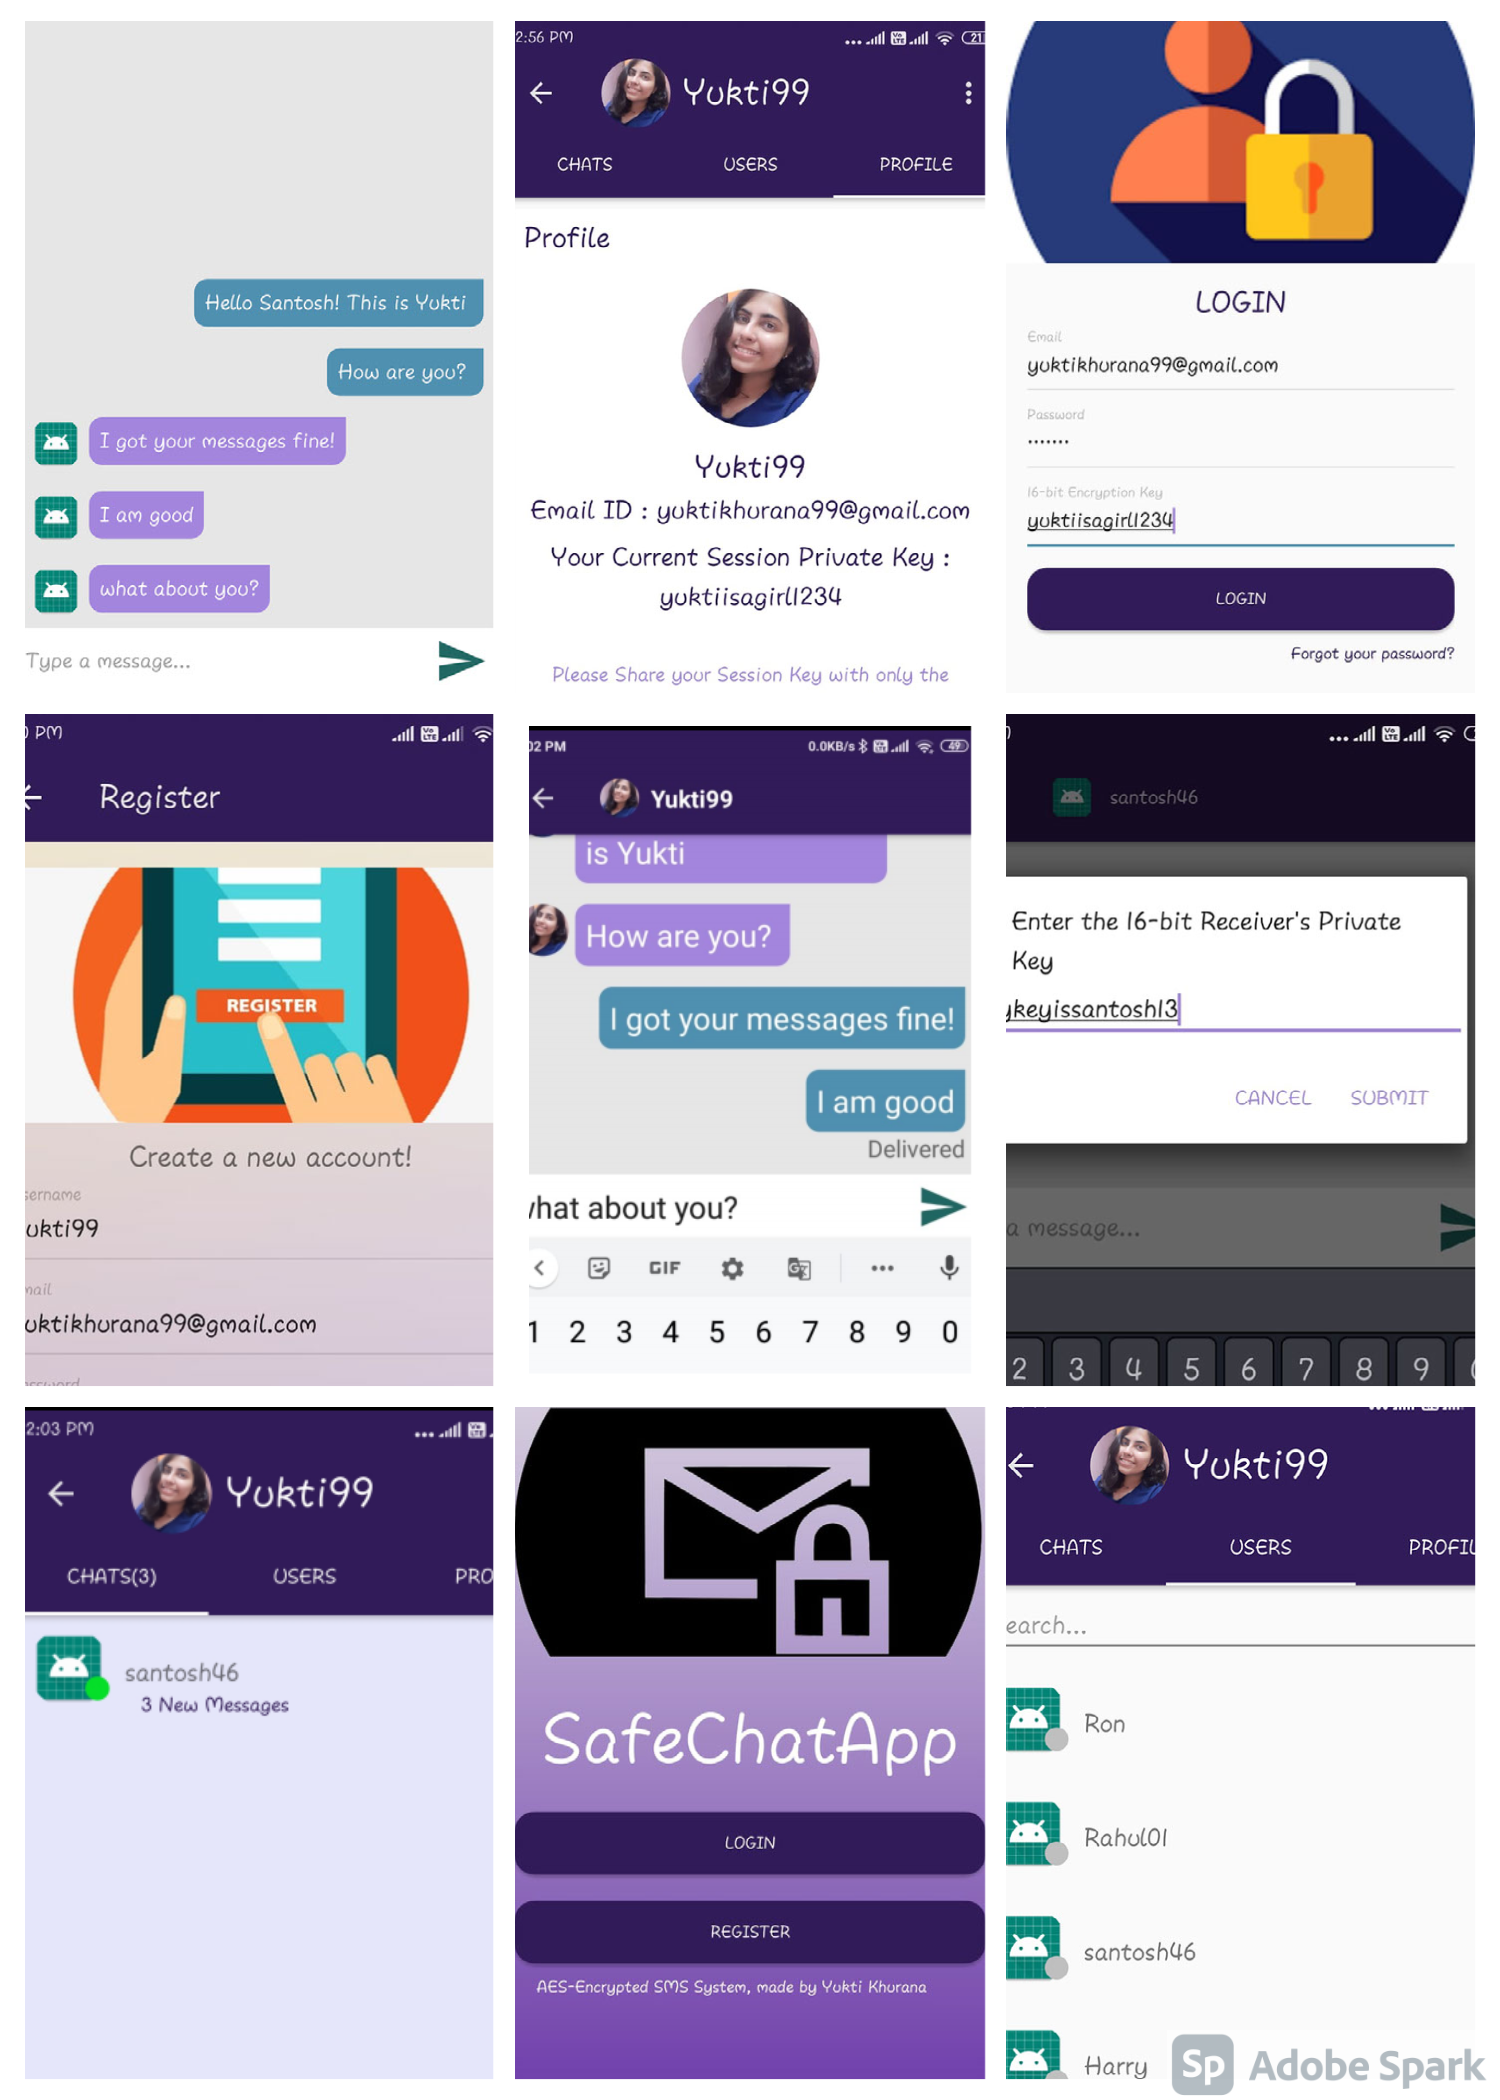
\includegraphics[width=.35\linewidth]{images/chatApp.jpeg}
  \caption{START PAGE }
  \label{fig:sub1}
\end{subfigure}
\end{figure}
\end{frame}

\begin{frame}
\begin{tcolorbox}
\begin{center}
\textsc{\textbf{\textcolor{byzantium}{THE SECURE CHATTING APP}}}
\end{center}
\end{tcolorbox}
\begin{figure}
\centering
\begin{subfigure}{\textwidth}
  \centering
  \includegraphics[width=.35\linewidth]{images/register.jpeg}
  \caption{REGISTER PAGE }
  \label{fig:sub1}
\end{subfigure}
\end{figure}
\end{frame}

\begin{frame}
\begin{tcolorbox}
\begin{center}
\textsc{\textbf{\textcolor{byzantium}{THE SECURE CHATTING APP}}}
\end{center}
\end{tcolorbox}
\begin{figure}
\centering
\begin{subfigure}{\textwidth}
  \centering
  \includegraphics[width=.35\linewidth]{images/login.jpeg}
  \caption{LOGIN PAGE }
  \label{fig:sub1}
\end{subfigure}
\end{figure}
\end{frame}


\begin{frame}
\begin{tcolorbox}
\begin{center}
\textsc{\textbf{\textcolor{byzantium}{HOW TO USE THE APP ?}}}
\end{center} 
\end{tcolorbox}
\begin{flushleft}
\begin{itemize}
\item The app opens up with a start-up page offering a choice between LOGIN or REGISTER.
\item To use the app, the user is required to first create an account using their email, a password with at least 6 characters and a username of their choice.
\item After successful registration, the user can login to the main activity page of the chat application.
\item For Login, the user must enter a 16-character encryption key to encrypt messages sent in the current logged in session. This key will act as the shared private key between the two interacting parties.
\end{itemize}
\end{flushleft}
\end{frame}

\begin{frame}
\begin{tcolorbox}
\begin{center}
\textsc{\textbf{\textcolor{byzantium}{Create an Account on MySafeChat App}}}
\end{center}
\end{tcolorbox}
\begin{figure}
\centering
\begin{subfigure}{\textwidth}
  \centering
  \includegraphics[width=.35\linewidth]{images/yregister.jpeg}
  \caption{1. Create your account by entering your email, a password and a username}
  \label{fig:sub1}
\end{subfigure}
\end{figure}
\end{frame}

\begin{frame}
\begin{tcolorbox}
\begin{center}
\textsc{\textbf{\textcolor{byzantium}{Login to your new Account}}}
\end{center}
\end{tcolorbox}
\begin{figure}
\centering
\begin{subfigure}{\textwidth}
  \centering
  \includegraphics[width=.35\linewidth]{images/ylogin.jpeg}
  \caption{2. Login to your account and enter the 16-character session key }
  \label{fig:sub1}
\end{subfigure}
\end{figure}
\end{frame}

\begin{frame}
\begin{tcolorbox}
\begin{center}
\textsc{\textbf{\textcolor{byzantium}{Home Page of your Account}}}
\end{center}
\end{tcolorbox}
\begin{figure}
\centering
\begin{subfigure}{\textwidth}
  \centering
  \includegraphics[width=.35\linewidth]{images/yprofile.jpeg}
  \caption{3. Profile Tab shows info about your profile, your username, session key, email and profile picture. You can change your username and pic in this }
  \label{fig:sub1}
\end{subfigure}
\end{figure}
\end{frame}



\begin{frame}
\begin{tcolorbox}
\begin{center}
\textsc{\textbf{\textcolor{byzantium}{BEGIN SECURE CHATTING}}}
\end{center} 
\end{tcolorbox}
\begin{center}
 \includegraphics[scale=0.08]{images/msglock.png}
\end{center}
\begin{flushleft}
\begin{itemize}
\item After successful login into the application, users may search from any users under the \textcolor{cyan}{“USERS”} tab of the home screen layout.
\item You can now normally text any of your friends or acquaintances.
\item The only catch is that as soon as you hit the send button your messages shall be encrypted using your current session private key that you entered during your login.
\item This will provide security to your chatting experience. 
\end{itemize}
\end{flushleft}
\end{frame}



\begin{frame}
\begin{tcolorbox}
\begin{center}
\textsc{\textbf{\textcolor{byzantium}{AT SENDER'S END}}}
\end{center}
\end{tcolorbox}
\begin{figure}
\centering
\begin{subfigure}{\textwidth}
  \centering
  \includegraphics[width=.35\linewidth]{images/yusers.jpeg}
  \caption{4.Users Tab, showing a list of all the users of the application  }
  \label{fig:sub1}
\end{subfigure}
\end{figure}
\end{frame}

\begin{frame}
\begin{tcolorbox}
\begin{center}
\textsc{\textbf{\textcolor{byzantium}{AT SENDER'S END}}}
\end{center}
\end{tcolorbox}
\begin{figure}
\centering
\begin{subfigure}{\textwidth}
  \centering
  \includegraphics[width=.35\linewidth]{images/ykey.jpeg}
  \caption{5.To chat with Santosh, enter her encryption Key  }
  \label{fig:sub1}
\end{subfigure}
\end{figure}
\end{frame}

\begin{frame}
\begin{tcolorbox}
\begin{center}
\textsc{\textbf{\textcolor{byzantium}{AT SENDER'S END}}}
\end{center}
\end{tcolorbox}
\begin{figure}
\centering
\begin{subfigure}{\textwidth}
  \centering
  \includegraphics[width=.35\linewidth]{images/ytext.jpeg}
  \caption{6.Once you send your message it is encrypted by your encryption key, in the background database, not visible to sender}
  \label{fig:sub1}
\end{subfigure}
\end{figure}
\end{frame}


\begin{frame}
\begin{tcolorbox}
\begin{center}
\textsc{\textbf{\textcolor{byzantium}{AT SENDER'S END}}}
\end{center}
\end{tcolorbox}
\begin{figure}
\centering
\begin{subfigure}{\textwidth}
  \centering
  \includegraphics[width=.35\linewidth]{images/ytext2.jpeg}
  \caption{7.The messages sent by Yukti are visible to herself for ease. It is also noted if the receiver has “SEEN” them yet or not}
  \label{fig:sub1}
\end{subfigure}
\end{figure}
\end{frame}


\begin{frame}
\begin{tcolorbox}
\begin{center}
\textsc{\textbf{\textcolor{byzantium}{AT SENDER'S END}}}
\end{center}
\end{tcolorbox}
\begin{figure}
\centering
\begin{subfigure}{\textwidth}
  \centering
  \includegraphics[width=.35\linewidth]{images/ychat.jpeg}
  \caption{8.Santosh added to your recent chat tab, so conversation can continue easily. }
  \label{fig:sub1}
\end{subfigure}
\end{figure}
\end{frame}


\begin{frame}
\begin{tcolorbox}
\begin{center}
\textsc{\textbf{\textcolor{byzantium}{AT RECEIVER'S END}}}
\end{center} 
\end{tcolorbox}
\begin{flushleft}
\begin{itemize}
\item As soon as the receiver logins into their account, they receive the notification of a message from a user. 
\item When the receiver clicks the chat to view the messages, they are prompted for the 16-character encryption key of the sender. 
\item Only if the user enters the correct key, can he read the decrypted message, otherwise, the message will seem just illegible gibberish. 
\item \textcolor{cyan}{This will provide further authorisation and privacy to both entities.}
On top of it, the messages sent by the receiver this time, will be encrypted using their distinct session key. So the sender must be aware of receiver’s key to read their messages.
\end{itemize}
\end{flushleft}
\end{frame}


\begin{frame}
\begin{tcolorbox}
\begin{center}
\textsc{\textbf{\textcolor{byzantium}{AT RECEIVER'S END}}}
\end{center}
\end{tcolorbox}
\begin{figure}
\centering
\begin{subfigure}{\textwidth}
  \centering
  \includegraphics[width=.35\linewidth]{images/9.jpeg}
  \caption{9.Santosh logs in using her account email and password, along with a session key }
  \label{fig:sub1}
\end{subfigure}
\end{figure}
\end{frame}


\begin{frame}
\begin{tcolorbox}
\begin{center}
\textsc{\textbf{\textcolor{byzantium}{AT RECEIVER'S END}}}
\end{center}
\end{tcolorbox}
\begin{figure}
\centering
\begin{subfigure}{\textwidth}
  \centering
  \includegraphics[width=.35\linewidth]{images/10.jpeg}
  \caption{10.Santosh’s Profile Information }
  \label{fig:sub1}
\end{subfigure}
\end{figure}
\end{frame}

\begin{frame}
\begin{tcolorbox}
\begin{center}
\textsc{\textbf{\textcolor{byzantium}{AT RECEIVER'S END}}}
\end{center}
\end{tcolorbox}
\begin{figure}
\centering
\begin{subfigure}{\textwidth}
  \centering
  \includegraphics[width=.35\linewidth]{images/11.jpeg}
  \caption{11.The messages received by Yukti are shown to Santosh on her home page}
  \label{fig:sub1}
\end{subfigure}
\end{figure}
\end{frame}


\begin{frame}
\begin{tcolorbox}
\begin{center}
\textsc{\textbf{\textcolor{byzantium}{AT RECEIVER'S END}}}
\end{center}
\end{tcolorbox}
\begin{figure}
\centering
\begin{subfigure}{\textwidth}
  \centering
  \includegraphics[width=.35\linewidth]{images/12.jpeg}
  \caption{12.To read the message sent by Yukti, Santosh (the receiver) must enter the encryption key of Yukti}
  \label{fig:sub1}
\end{subfigure}
\end{figure}
\end{frame}


\begin{frame}
\begin{tcolorbox}
\begin{center}
\textsc{\textbf{\textcolor{byzantium}{AT RECEIVER'S END}}}
\end{center}
\end{tcolorbox}
\begin{figure}
\centering
\begin{subfigure}{\textwidth}
  \centering
  \includegraphics[width=.35\linewidth]{images/13.jpeg}
  \caption{13.Now, Santosh can read Yukti’s messages! }
  \label{fig:sub1}
\end{subfigure}
\end{figure}
\end{frame}


\begin{frame}
\begin{tcolorbox}
\begin{center}
\textsc{\textbf{\textcolor{byzantium}{SECURE CONVERSATIONS USING AES}}}
\end{center}
\end{tcolorbox}
\begin{figure}
\centering
\begin{subfigure}{\textwidth}
  \centering
  \includegraphics[width=.35\linewidth]{images/14.jpeg}
  \caption{14.Now, Santosh can continue the conversation in a similar way }
  \label{fig:sub1}
\end{subfigure}
\end{figure}
\end{frame}

\begin{frame}
\begin{tcolorbox}
\begin{center}
\textsc{\textbf{\textcolor{byzantium}{SECURE CONVERSATIONS USING AES}}}
\end{center}
\end{tcolorbox}
\begin{figure}
\centering
\begin{subfigure}{\textwidth}
  \centering
  \includegraphics[width=.35\linewidth]{images/15.jpeg}
  \caption{15.But the messages sent by Santosh will be encrypted using her session key. }
  \label{fig:sub1}
\end{subfigure}
\end{figure}
\end{frame}

\begin{frame}
\begin{tcolorbox}
\begin{center}
\textsc{\textbf{\textcolor{byzantium}{SECURE CONVERSATIONS USING AES}}}
\end{center}
\end{tcolorbox}
\begin{figure}
\centering
\begin{subfigure}{\textwidth}
  \centering
  \includegraphics[width=.35\linewidth]{images/16.jpeg}
  \caption{16.Yukti will receive notification of Santosh’s messages and shall user her key to read them }
  \label{fig:sub1}
\end{subfigure}
\end{figure}
\end{frame}

\begin{frame}
\begin{tcolorbox}
\begin{center}
\textsc{\textbf{\textcolor{byzantium}{SECURE CONVERSATIONS USING AES}}}
\end{center}
\end{tcolorbox}
\begin{figure}
\centering
\begin{subfigure}{\textwidth}
  \centering
  \includegraphics[width=.35\linewidth]{images/17.jpeg}
  \caption{17.Yukti will type Santosh’s encryption key }
  \label{fig:sub1}
\end{subfigure}
\end{figure}
\end{frame}

\begin{frame}
\begin{tcolorbox}
\begin{center}
\textsc{\textbf{\textcolor{byzantium}{SECURE CONVERSATIONS USING AES}}}
\end{center}
\end{tcolorbox}
\begin{figure}
\centering
\begin{subfigure}{\textwidth}
  \centering
  \includegraphics[width=.35\linewidth]{images/18.jpeg}
  \caption{18.Now, Yukti can read Santosh’s messages easily and securely! }
  \label{fig:sub1}
\end{subfigure}
\end{figure}
\end{frame}

\begin{frame}
\begin{tcolorbox}
\begin{center}
\textsc{\textbf{\textcolor{byzantium}{WHAT IF THE WRONG KEY IS ENTERED?}}}
\end{center}
\end{tcolorbox}
\begin{figure}
\centering
\begin{subfigure}{\textwidth}
  \centering
  \includegraphics[width=.35\linewidth]{images/19.jpeg}
  \caption{19.Suppose the receiver enters a wrong key}
  \label{fig:sub1}
\end{subfigure}
\end{figure}
\end{frame}

\begin{frame}
\begin{tcolorbox}
\begin{center}
\textsc{\textbf{\textcolor{byzantium}{WHAT IF THE WRONG KEY IS ENTERED?}}}
\end{center}
\end{tcolorbox}
\begin{figure}
\centering
\begin{subfigure}{\textwidth}
  \centering
  \includegraphics[width=.35\linewidth]{images/20.jpeg}
  \caption{20.The receiver won’t be able to read the received messages, it will seem like all gibberish.}
  \label{fig:sub1}
\end{subfigure}
\end{figure}
\end{frame}





\begin{frame}
\begin{tcolorbox}
\begin{center}
\textsc{\textbf{\textcolor{byzantium}{BACK-END FIREBASE DATABASE}}}
\end{center}
\end{tcolorbox}
\begin{flushleft}
\begin{itemize}
\item Firebase online database has been used to store information about the app.
\item The users table as shown created in the firebase whenever a user creates an account on SafeChatApp. providing the communication service, has knowledge of the encryption keys.
\item The user information stored is: id, username, image url, status and search.
\end{itemize}
\end{flushleft}
\end{frame}

\begin{frame}
\begin{tcolorbox}
\begin{center}
\textsc{\textbf{\textcolor{byzantium}{BACK-END FIREBASE DATABASE}}}
\end{center}
\end{tcolorbox}
\begin{center}
\includegraphics[scale=0.35]{images/users.PNG}
\end{center}
\end{frame}

\begin{frame}[plain]
\begin{tcolorbox}
\begin{center}
\textsc{\textbf{\textcolor{byzantium}{CHATS STORED IN ENCRYPTED FORM}}}
\end{center}
\end{tcolorbox}
\begin{figure}
\centering
\begin{subfigure}{\textwidth}
  \centering
  \includegraphics[scale=0.27]{images/chats.PNG}
  \caption{The chats are stored in encrypted for, so even the communication provider cannot eavesdrop}
  \label{fig:sub1}
\end{subfigure}
\end{figure}
\end{frame}

\begin{frame}
\begin{tcolorbox}
\begin{center}
\textsc{\textbf{\textcolor{byzantium}{ENCRYPTED CHATS}}}
\end{center}
\end{tcolorbox}
\begin{flushleft}
\begin{itemize}
\item The chats stored in Chats Table of the SMS-encryption database, stores all the information in encrypted form..
\item The sender and receiver’s id is stored, to reload previous conversations at a later time.
\item The message is stored in encrypted form so that there is complete privacy between sender and receiver and even the communication provider cannot read/ eavesdrop the conversation.
\end{itemize}
\end{flushleft}
\end{frame}

\begin{frame}
\begin{tcolorbox}
\begin{center}
\textsc{\textbf{\textcolor{byzantium}{ENCRYPTED CHATS}}}
\end{center}
\end{tcolorbox}
\begin{center}
\includegraphics[scale=0.45]{images/chatslist.PNG}
\end{center}
\end{frame}


\begin{frame}
\begin{tcolorbox}
\begin{center}
\textsc{\textbf{\textcolor{byzantium}{MORE FEATURES OF THE APP}}}
\end{center} 
\end{tcolorbox}
\begin{flushleft}
\begin{itemize}
\item The SafeChatApp is very convenient to use and provided complete end-to-end encryption.  
\item The added security measure of prompting the receiver for encryption key provides \textcolor{purple} { authentication, confidentiality as well as integrity}.This app ensures that no malicious entity or hacker can steal private conversation information without knowing the key.
\item Further security measure employed in this android app is the fact that, each side has its own private key i.e. to read the whole conversation and make sense out of it, the attacker must have the keys of both parties.
\item \textcolor{purple} {The Key is session-dependent}, i.e. in each session the user can choose any key of his/her choice. 
\item The communication-providing entity i.e. SafeChatApp will have no information about the key. \textcolor{purple} {If a user wants, he can change the key for a new session, this will render all the previous conversation unreadable and thus untraceable.}
\end{itemize}
\end{flushleft}
\end{frame}


\begin{frame}
\begin{tcolorbox}
\begin{center}
\textsc{\textbf{\textcolor{byzantium}{TECHNICAL DETAILS OF THE APP}}}
\end{center} 
\end{tcolorbox}
\begin{flushleft}
\begin{itemize}
\item \textcolor{cyan}{NAME}: SafeChatApp
\item \textcolor{cyan}{BACKEND}: Java 
\item \textcolor{cyan}{FRONTEND}: XML
\item \textcolor{cyan}{SOFTWARE}: Android Studio on Windows 10
\item \textcolor{cyan}{ANDROID STUDIO VERSION}: 3.4.2
\item \textcolor{cyan}{DATABASE}:Firebase Database \& Storage
\item \textcolor{cyan}{MINIMUM SDK VERSION}: 16
\item \textcolor{cyan}{TARGET SDK VERSION}: 28 
\item \textcolor{cyan}{APP PERMISSIONS}: Internet Connection, Device’s External Storage read/write permissions
\item \textcolor{cyan}{ABOUT}: App works perfectly on 84.5\% of android devices of matching SDK configurations
\end{itemize}
\end{flushleft}
\end{frame}

\begin{frame}
\begin{tcolorbox}
\begin{center}
\textsc{\textbf{\textcolor{byzantium}{AES ENCRYPTION & DECRYPTION}}}
\end{center} 
\end{tcolorbox}
\begin{flushleft}
\begin{itemize}
\item The app uses Advanced Encryption Standard to encrypt and decrypt the messages exchanged between the users.
\item AES is one of the most popular and widely adopted symmetric encryption algorithm. It is at  least 6 times faster than Triple DES.
\item It is a symmetric block cipher that encrypts data in blocks of size 128-bit and uses 128/192/256 keys for encryption.
\item The large size of AES keys and multiple rounds of substitution and permutation make it a very strong encryption standard which has not been broken by any known person till now. 
\item AES-256 with 256 bit key and 14-rounds is the most advance cryptographic algorithm till date and not have been broken yet.
\item It is a symmetric block cipher i.e. the same key is used to encrypt and decrypt the plaintext or message. So both sender and receiver must know the same secret key.
\end{itemize}
\end{flushleft}
\end{frame}

\begin{frame}[plain]
\begin{tcolorbox}
\begin{center}
\textsc{\textbf{\textcolor{byzantium}{AES ENCRYPTION & DECRYPTION}}}
\end{center} 
\end{tcolorbox}
\begin{center}
\includegraphics[scale=0.28]{images/aes.png}
\end{center}
\end{frame}


\begin{frame}
\begin{tcolorbox}
\begin{center}
\textsc{\textbf{\textcolor{byzantium}{WHY AND HOW AES MAKES THE APP SECURE?}}}
\end{center} 
\end{tcolorbox}
\begin{flushleft}
\begin{itemize}
\item Its building blocks and design principles are fully specified.
\item It has sustained years of attempted cryptanalysis from many smart people, in a high-exposure situation, and it came out relatively unscathed.
\item AES makes extensive use of Galois field theory
\item AES being a symmetric key algorithm is not known to be reduced to any “known hard problem” which makes it unbreakable for current computational speeds.
\itemThe best key-recovery attacks on full AES so far is a Biclique attack which is merely faster than brute force by at most a factor of 4. Furthermore, the data storage required works out to trillions of terabytes, far beyond the data stored on the planet.
\item The strength of AES increases exponentially with Key-size as it leads to more “Confusion”- an important property of any secure cipher.
\end{itemize}
\end{flushleft}
\end{frame}

\begin{frame}[plain]
\begin{tcolorbox}
\begin{center}
\textsc{\textbf{\textcolor{byzantium}{MY APP'S BACKGROUND ENCRYPTION \& DECRYPTION LOGIC}}}
\end{center} 
\end{tcolorbox}
\begin{center}
\includegraphics[scale=0.62]{images/AES-APP-LOGIC.PNG}
\end{center}
\end{frame}

\begin{frame}
\begin{tcolorbox}
\begin{center}
\textsc{\textbf{\textcolor{byzantium}{BACKEND LOGIC FOR AES ENCRYPTION}}}
\end{center}
\end{tcolorbox}
\begin{figure}
\centering
\begin{subfigure}{\textwidth}
  \centering
   \begin{center}
  \caption{
  Java cryptography architecture is used here and the sender’s key is the current-session private key used for encryption in the send-message function of MessageActivity Module of the app.}
  \end{center}
  \includegraphics[width=9.5cm,height=6.2cm]{images/c1.PNG}
  \label{fig:sub1}
\end{subfigure}
\end{figure}
\end{frame}


\begin{frame}
\begin{tcolorbox}
\begin{center}
\textsc{\textbf{\textcolor{byzantium}{SEND MESSAGE FUNCTION AT SENDER'S END}}}
\end{center}
\end{tcolorbox}
\begin{figure}
\centering
\begin{subfigure}{\textwidth}
  \centering
   \begin{center}
  \caption{
  The send message function of the MessageActivity module encrypts the message using AESEncryptionMethod() function and then stores encrypted data to firebase database instead of the real data.}
  \end{center}
  \includegraphics[width=9.5cm,height=6.2cm]{images/c2.PNG}
  \label{fig:sub1}
\end{subfigure}
\end{figure}
\end{frame}


\begin{frame}
\begin{tcolorbox}
\begin{center}
\textsc{\textbf{\textcolor{byzantium}{AES ENCRYPTION METHOD AT SENDER'S END}}}
\end{center}
\end{tcolorbox}
\begin{figure}
\centering
\begin{subfigure}{\textwidth}
  \centering
    \begin{center}
  \caption{
  The message is first converted to a byte array and then encrypt mode and secretKeySpec are created using sender’s session key.The standard use here is ISO-8859-1,but any other can also be used.}
  \end{center}
  \includegraphics[width=9.5cm,height=6.2cm]{images/c3.PNG}

  \label{fig:sub1}
\end{subfigure}
\end{figure}
\end{frame}

\begin{frame}
\begin{tcolorbox}
\begin{center}
\textsc{\textbf{\textcolor{byzantium}{READ MESSAGE FUNCTION AT RECEIVER'S END}}}
\end{center}
\end{tcolorbox}
\begin{figure}
\centering
\begin{subfigure}{\textwidth}
  \centering
  \includegraphics[width=10cm,height=7cm]{images/c4.PNG}
  \begin{flushleft}
  \end{flushleft}
  \label{fig:sub1}
\end{subfigure}
\end{figure}
\end{frame}

\begin{frame}
\begin{tcolorbox}
\begin{center}
\textsc{\textbf{\textcolor{byzantium}{READ MESSAGE FUNCTION AT RECEIVER'S END}}}
\end{center} 
\end{tcolorbox}
\begin{flushleft}
\begin{itemize}
\item The read message function of the MessageActivity module of app, first prompts the user to enter a 16-character encryption key of the sender.
\item The same key is converted to AES key standard and used to decrypt the encrypted message retrieved from the firebase database. 
\item If the key is correct, the message will be decrypted correctly.For the sender reading his sent messages, the messages are decoded already for him to read easily. 
\end{itemize}
\end{flushleft}
\end{frame}



\begin{frame}
\begin{tcolorbox}
\begin{center}
\textsc{\textbf{\textcolor{byzantium}{AES DECRYPTION METHOD AT RECEIVER'S END}}}
\end{center}
\end{tcolorbox}
\begin{figure}
\centering
\begin{subfigure}{\textwidth}
  \centering
    \begin{center}
  \caption{
This function returns the decrypted version of the encrypted message given, using the key provided by the receiver.If the key is entered correctly by the receiver, the data will be decrypted correctly and user will be able to read it.}
  \end{center}
  \includegraphics[width=9.5cm,height=6.0cm]{images/c5.PNG}

  \label{fig:sub1}
\end{subfigure}
\end{figure}
\end{frame}


\begin{frame}
\begin{tcolorbox}
\begin{center}
\textsc{\textbf{\textcolor{byzantium}{CONCLUSION}}}
\end{center}
\end{tcolorbox}
\begin{flushleft}
\begin{itemize}
\item Given the exceptional strength of AES Algorithm, This android app will ensure  a secure chatting experience for users who don’t want their conversations to be eavesdropped by any third entity. 
\item Every user session is end-to-end encrypted in such a manner that there is not inconvenience to the user. 
\item The users communicating must enter their session-encryption keys that both of them must be aware of and they can start messaging!
\end{itemize}
\end{flushleft}
\end{frame}


\begin{frame}
\begin{center}
\begin{tcolorbox}
\begin{center}
\textsc{\textbf{\textcolor{byzantium}{\huge THANK YOU}}}
\end{center}
\end{tcolorbox}
\begin{center}
\textcolor{pink}{
CYBER-SECURITY/ COMPUTER NETWORKS AND SECURITY PROJECT \linebreak
MADE BY YUKTI KHURANA \linebreak
2017UCP1234 \linebreak
6TH SEMESTER, 3RD YEAR BTECH \linebreak
MALAVIYA NATIONAL INSTITUTE OF TECHNOLOGY, JAIPUR \linebreak
}
\end{center}
\end{center}
\end{frame}

\end{document}
